\section{Graph isomorphism}

In Example \ref{exm:npc} we mentioned that graph isomorphism problem is assumed to be neither $\P$ nor $\NP$-complete. From this reason it seems to belong to a special class and thus we will describe a DNA system which solves this very special problem. %!% vocitovat

Following approach is very similar to 3-coloring if we consider $n$ colors instead. The problem can be stated: ``For a non-colored graph $G$ and a graph $H$ where every vertex is colored with different color, find a coloring of $G$ with all of those $n$ colors used exactly once (1) such that these colored graphs are isomorphic (2).'' Now one has to check that:
\begin{enumerate}
	\item every ``color'' was used exactly once so that it is a bijection,
	\item edges and non-edges are preserved.
\end{enumerate}

\subsection*{Set of tiles}

Like before, the graph needs to have even number of vertices, thus one separated self-bijective vertex has to be added if applicable. An example is given, see Figure \ref{fig:graph_iso}.
\begin{description}
	\item[Bottom line] These tiles have almost exactly the same rules as in graph 3-coloring, the difference is that {\em all} of the same-colored combinations are omitted. $\frac{n^3}{2}$ tile types were required.
	\item[Bottom corner tiles] Are exactly the same. $2$ tile types were required.
	\item[Inner tiles] There are three types of inner tiles:
	\begin{description}
		\item[Number-ordering tiles] These are similar to previous ones, the difference is which do exist and which do not. Let us assume a tile with numbers $k$ and $l$ with colors $a$ and $b$, respectively. Note that numbers $k$ and $l$ correspond with vertices in graph $G$ and colors $a$ and $b$ correspond with vertices in graph $H$. This tile must check the isomorphism property -- existence or non-existence of edge between appropriate vertices. Thus the tile exists if and only if
		$$(\{k,\,l\} \in E(G) \wedge \{a,\,b\} \in E(H)) \vee (\{k,\,l\} \notin E(G) \wedge \{a,\,b\} \notin E(H)) . $$
		From similar reasons all pairs of vertices from graph $G$ meet each other, thus every edge is checked so condition number $2$ would be done. $n^4$ tile types were required.
		\item[Color extracting tiles] Now we have to extract colors (forget numbers) and order them in given order so that we can check that every color is used exactly once. This process will be triggered by a special inner tile with the highest number of arbitrary color and a non-colored asterisk on the bottom. On the top it will have an asterisk of that number's color and a non-colored asterisk. For every other number with arbitrary color there exists a tile with it and an asterisk of an arbitrary but different color on the bottom. On the top it will have two asterisks of these colors in correct order. $n^3$ tile types were required.
		\item[Color-ordering tiles] These are similar to those with numbers. Similarly there do not exist tiles with one color. $n^2$ tile types were required.
		% there is some redundancy .. but no idea how to do it faster .. it can be done easier, one can only check without colors, same colors are killed during ordering!
	\end{description}
	\item[Border tiles] These tiles are exactly the same like for 3-coloring.
	\item[Checking tiles] As soon as there appears a combination of sharp and most-left-colored asterisk, a checking tile comes having ``C'' of the second color on the right top. After this initialization there are tiles with colored ``C'' and same-colored asterisk on the bottom and next-colored ``C'' on the right top. This ensures that every color was used exactly once. The last color is followed by non-colored ``C''. $n$ tile types were required.
	\item[DONE tile] Finally if non-colored ``C'' meets non-colored asterisk, a ``DONE'' tile is connected signalizing correct solution. $1$ tile type was required.
\end{description}
Summed up, this DNA algorithm requires $n^4$ tile types and its binding complexity is $2\nicefrac{1}{2}\;n^2$. Glue complexity is ...

% .. místo na trik

\begin{figure}[H]
\begin{center}
	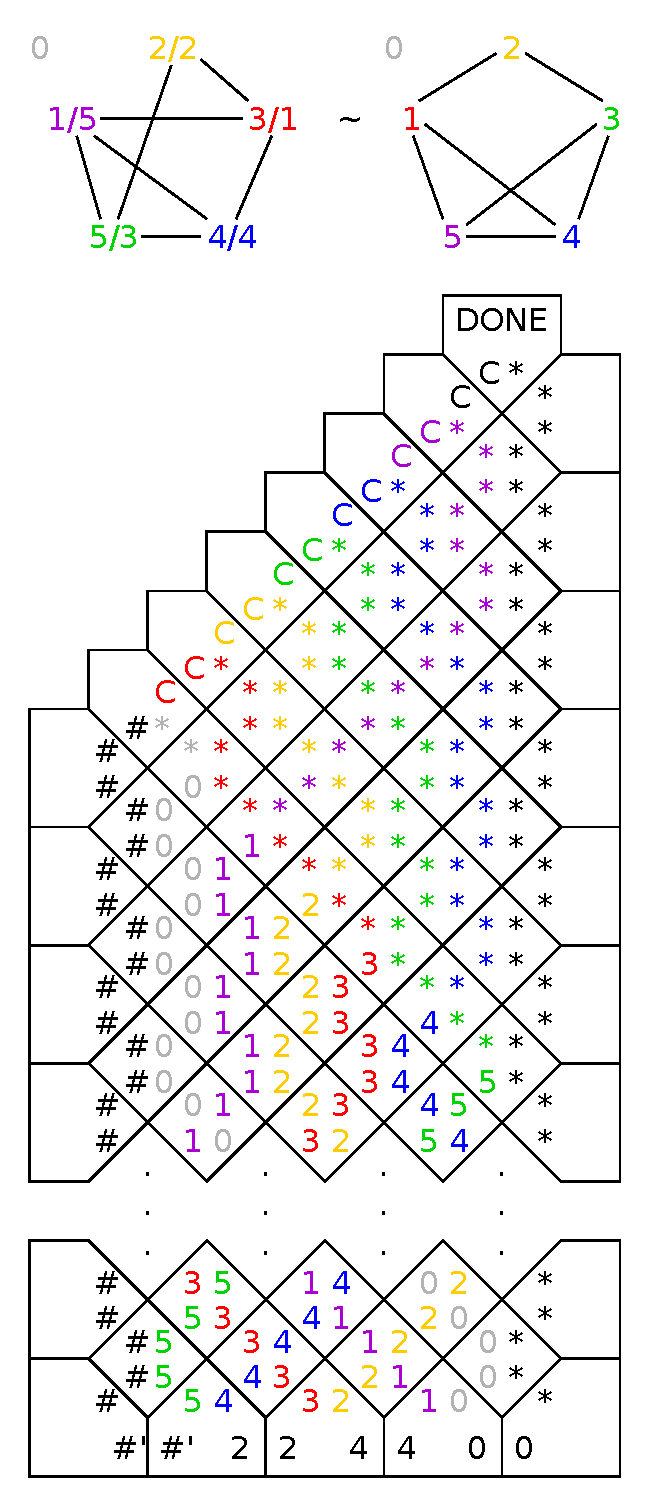
\includegraphics[scale=0.75]{./figures/isomorphism/isomorphism.pdf}
	\caption{Graph isomorphism computation. Color order is defined by their wavelength.}
	\label{fig:graph_iso}
\end{center}
\end{figure}
